\documentclass[../AnalysisNoteJBuxton.tex]{subfiles}
\begin{document}

\subsection{V0 Selection}
\label{V0Selection}

$\Lambda$ ($\bar{\Lambda}$) and K$^{0}_{S}$ are neutral particles which cannot be directly detected, but must instead be reconstructed through detection of their decay products, or daughters.  
In general, particles which are topologically reconstructed in this fashion are called V0 particles.
The class AliFemtoV0TrackCutNSigmaFilter (which is an extension of AliFemtoV0TrackCut) is used to reconstruct the V0s.

\begin{figure}[h]
  \centering
  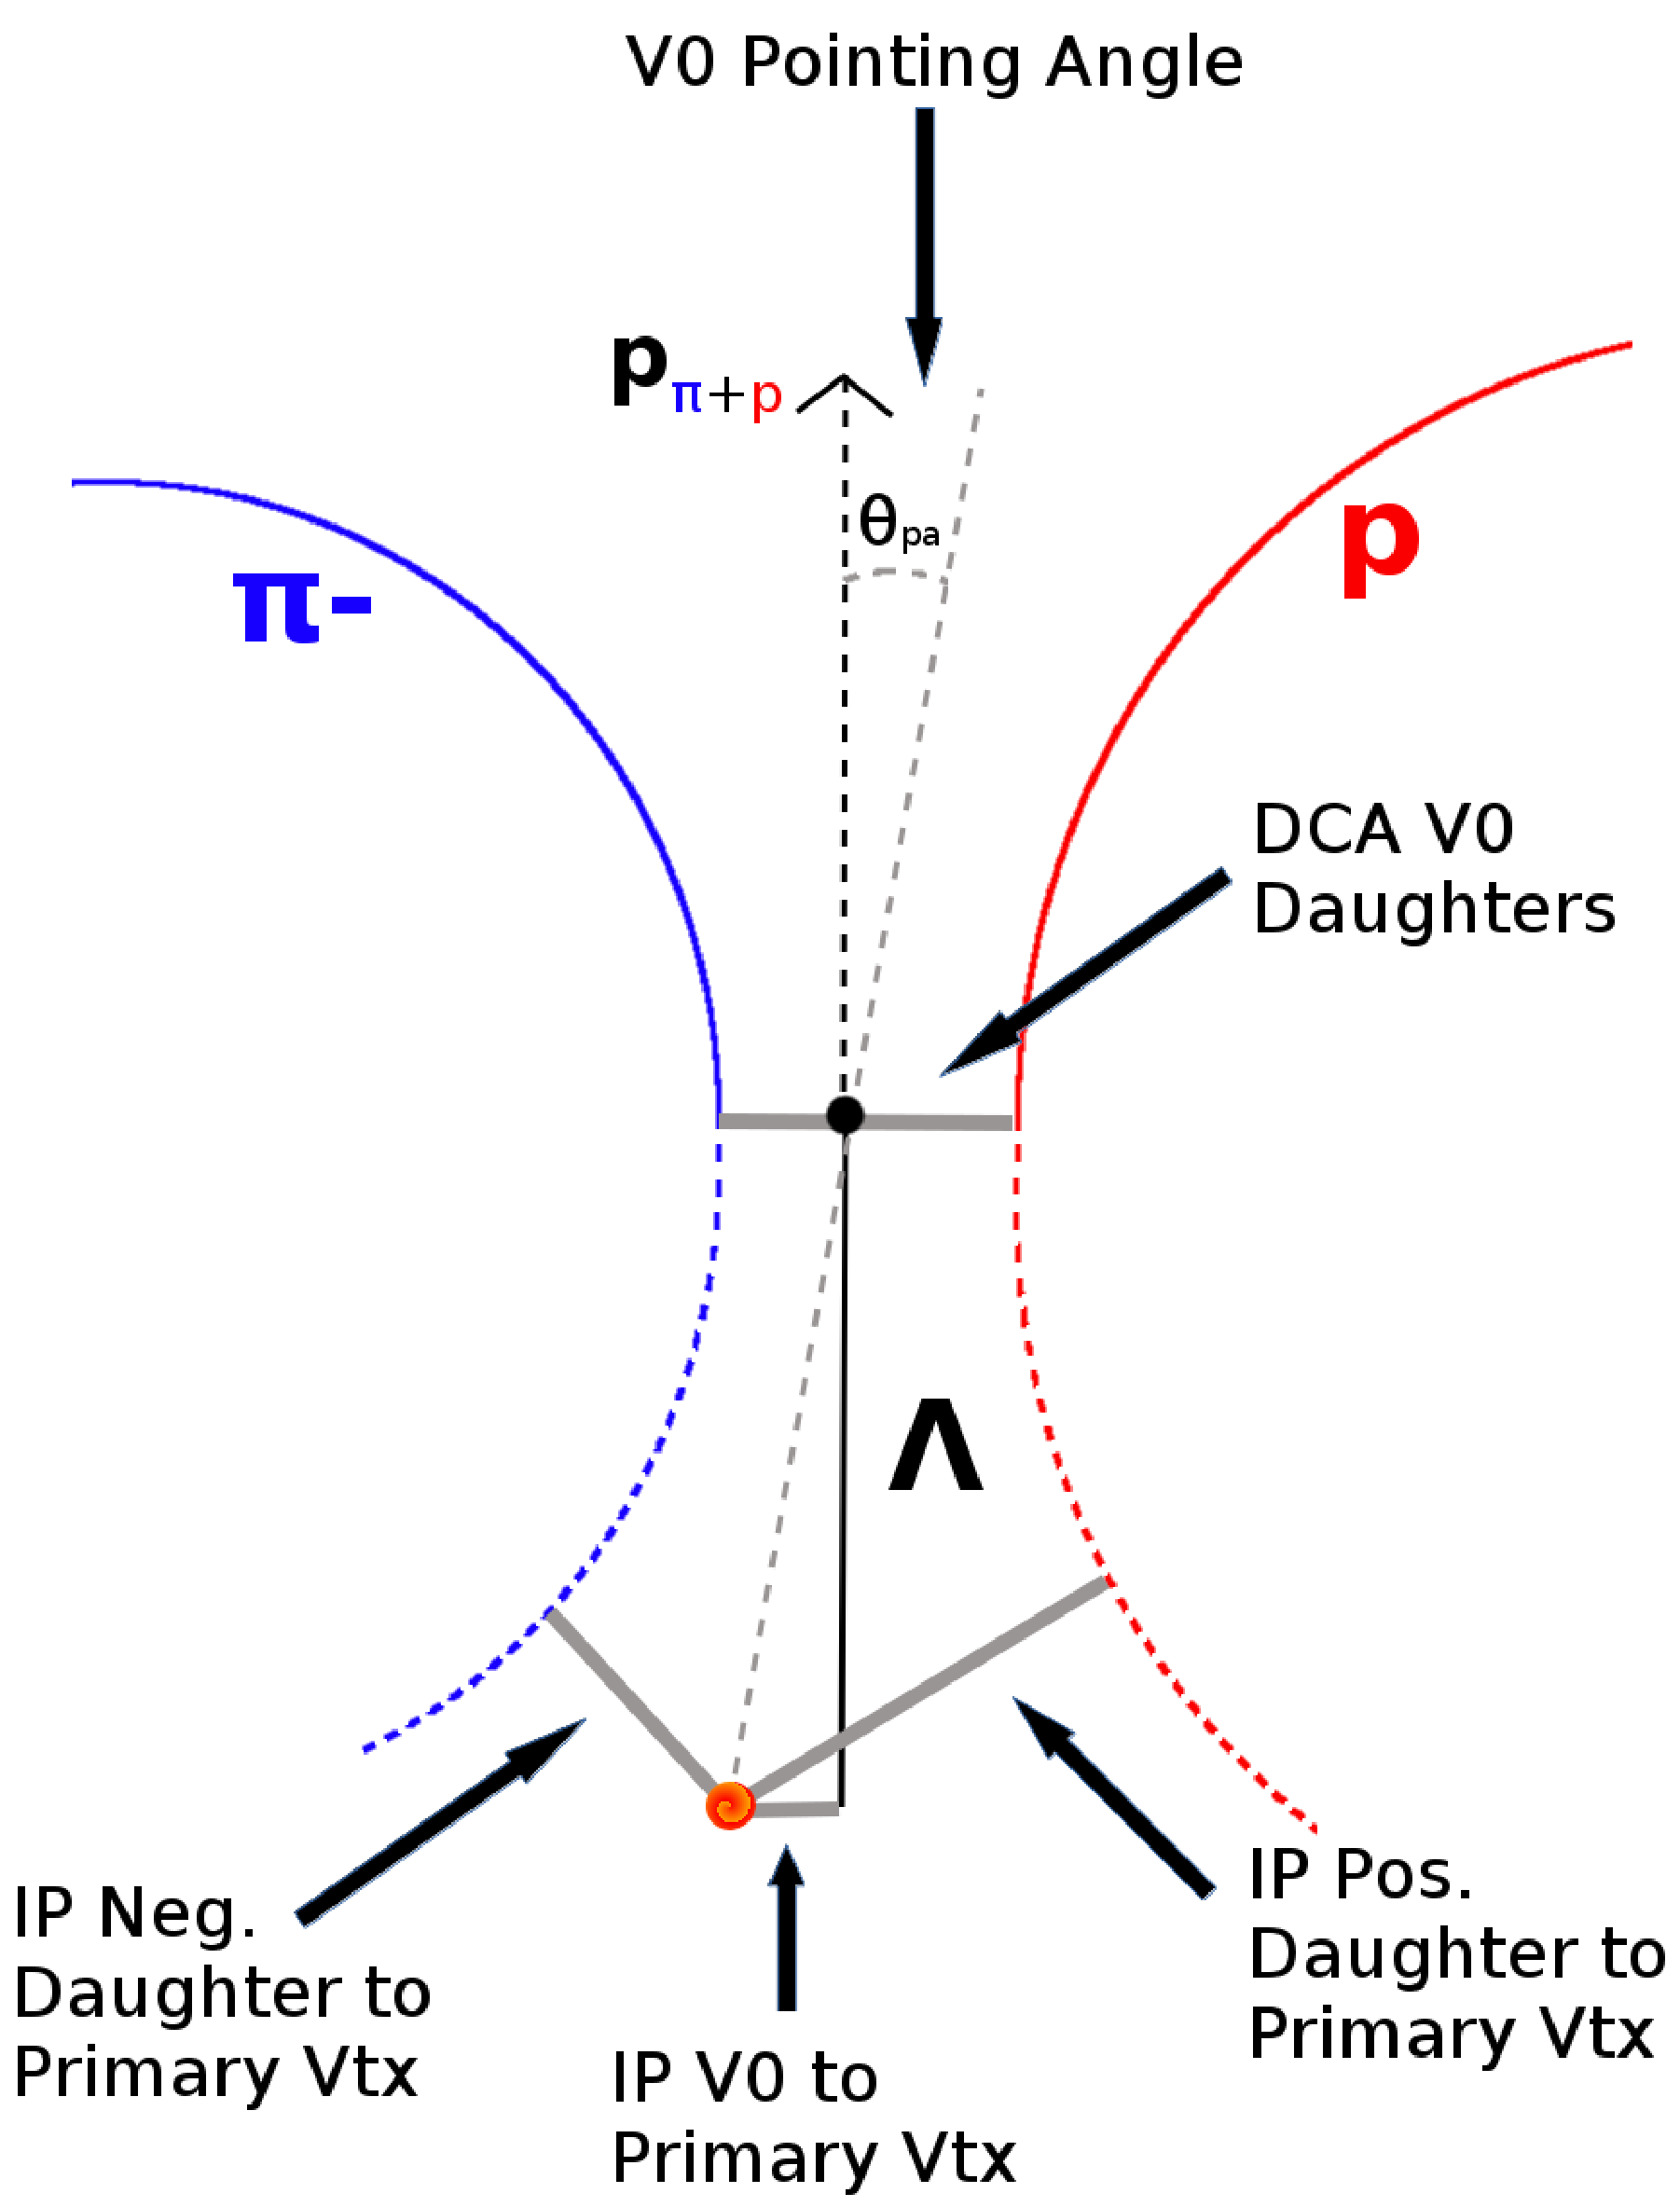
\includegraphics[width=100mm]{3_DataSelection/Figures/V0Cuts.pdf}
  \caption[$\Lambda$ Reconstruction]{$\Lambda$ Reconstruction}
  \label{fig:LamReconstruction}
\end{figure}

\begin{figure}[h]
  \centering
  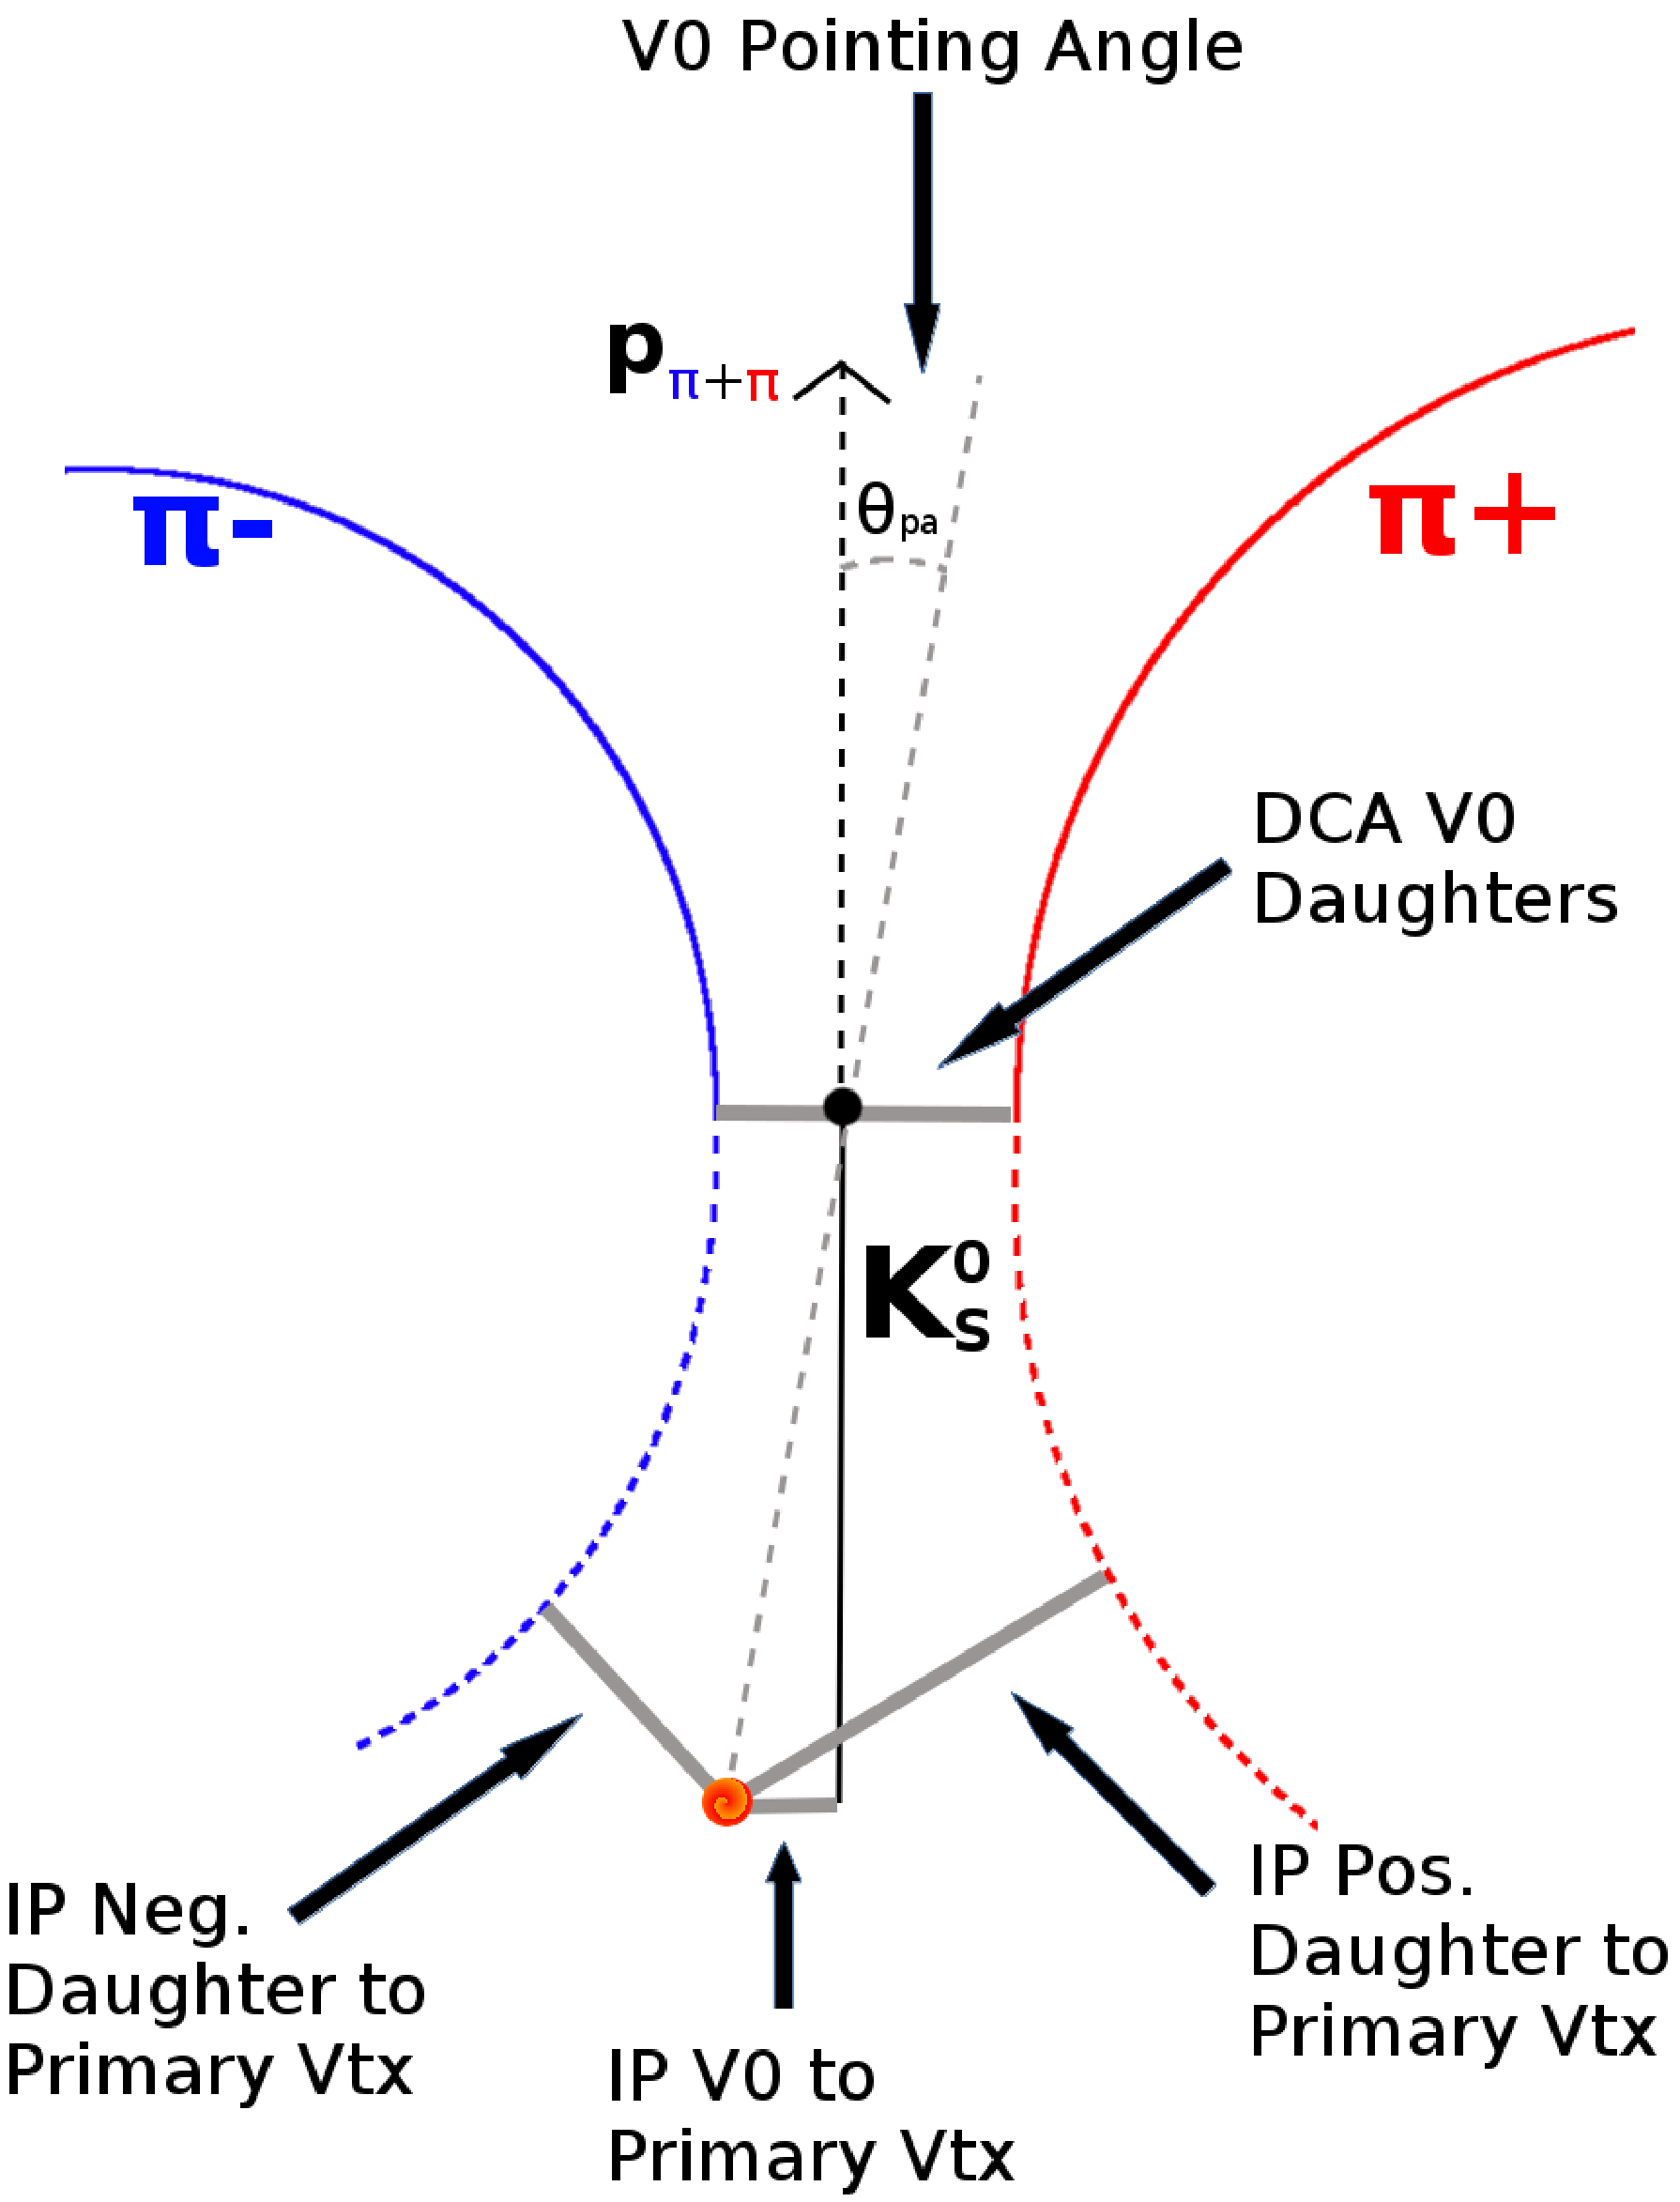
\includegraphics[width=100mm]{3_DataSelection/Figures/K0Cuts.pdf}
  \caption[K$^{0}_{S}$ Reconstruction]{K$^{0}_{S}$ Reconstruction}
  \label{fig:K0Reconstruction}
\end{figure}


\begin{figure}[h]
\begin{minipage}{18pc}
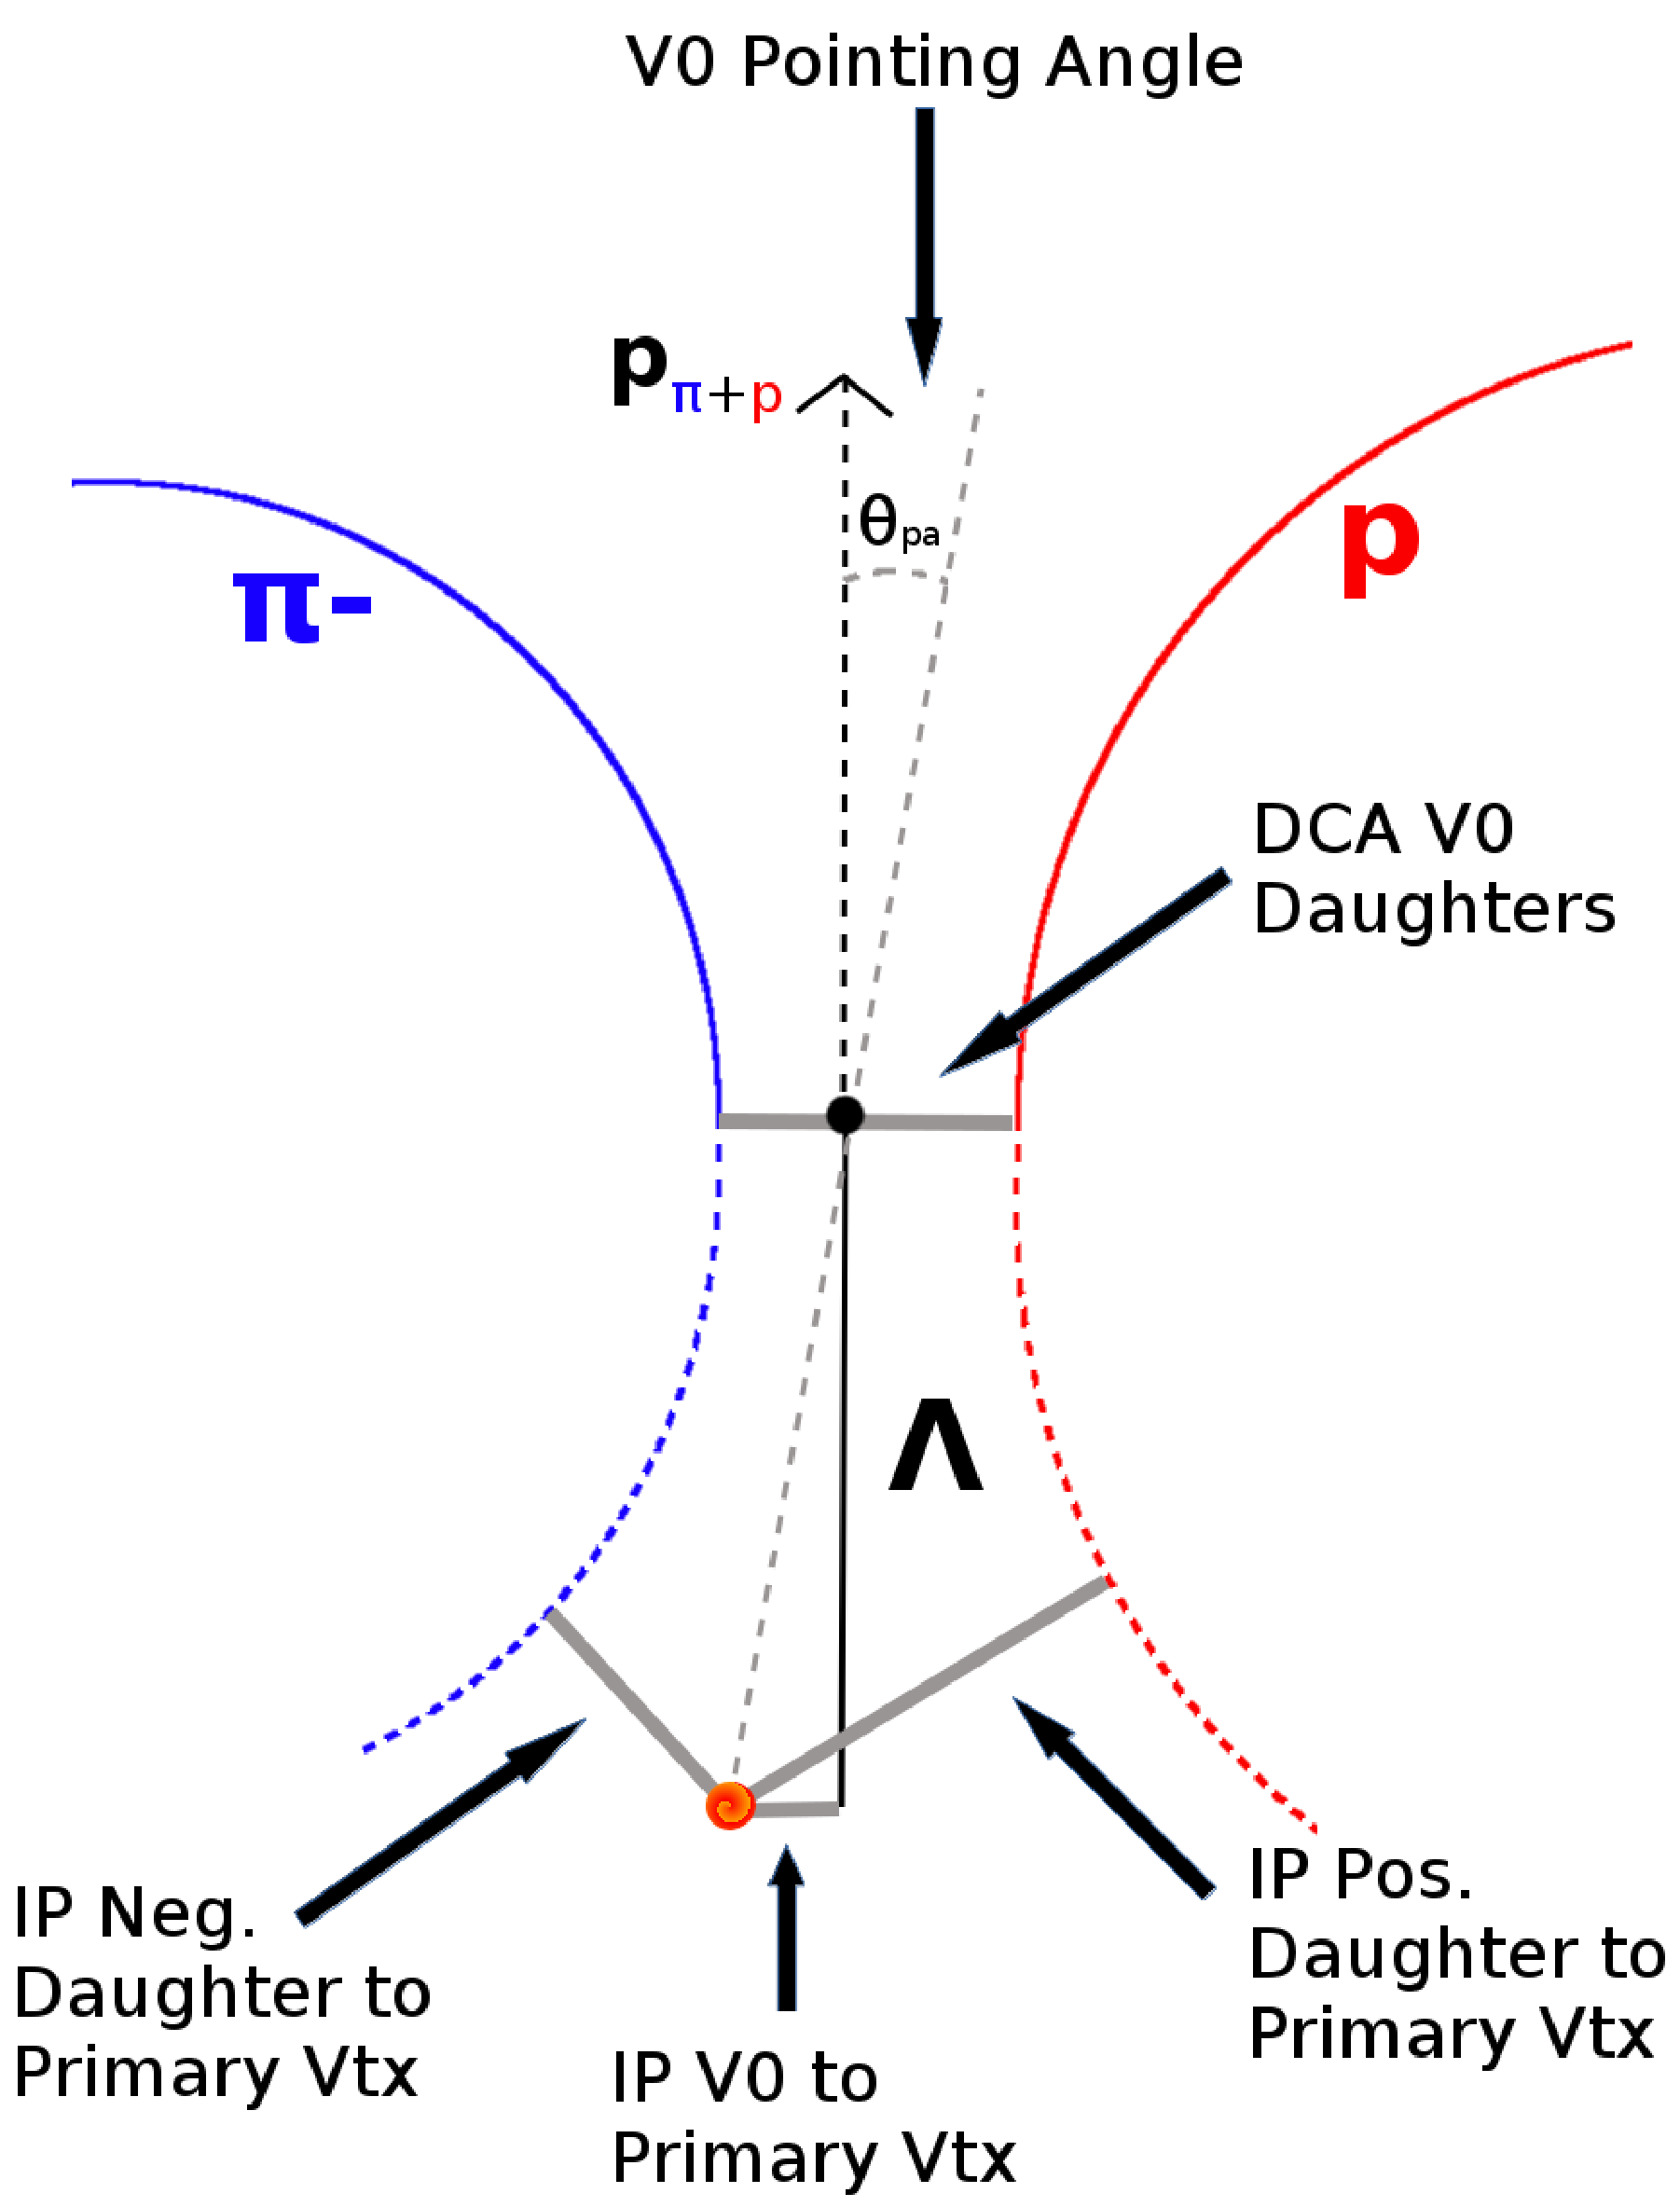
\includegraphics[width=18pc]{3_DataSelection/Figures/V0Cuts.pdf}
\end{minipage}\hspace{2pc}
\begin{minipage}{18pc}
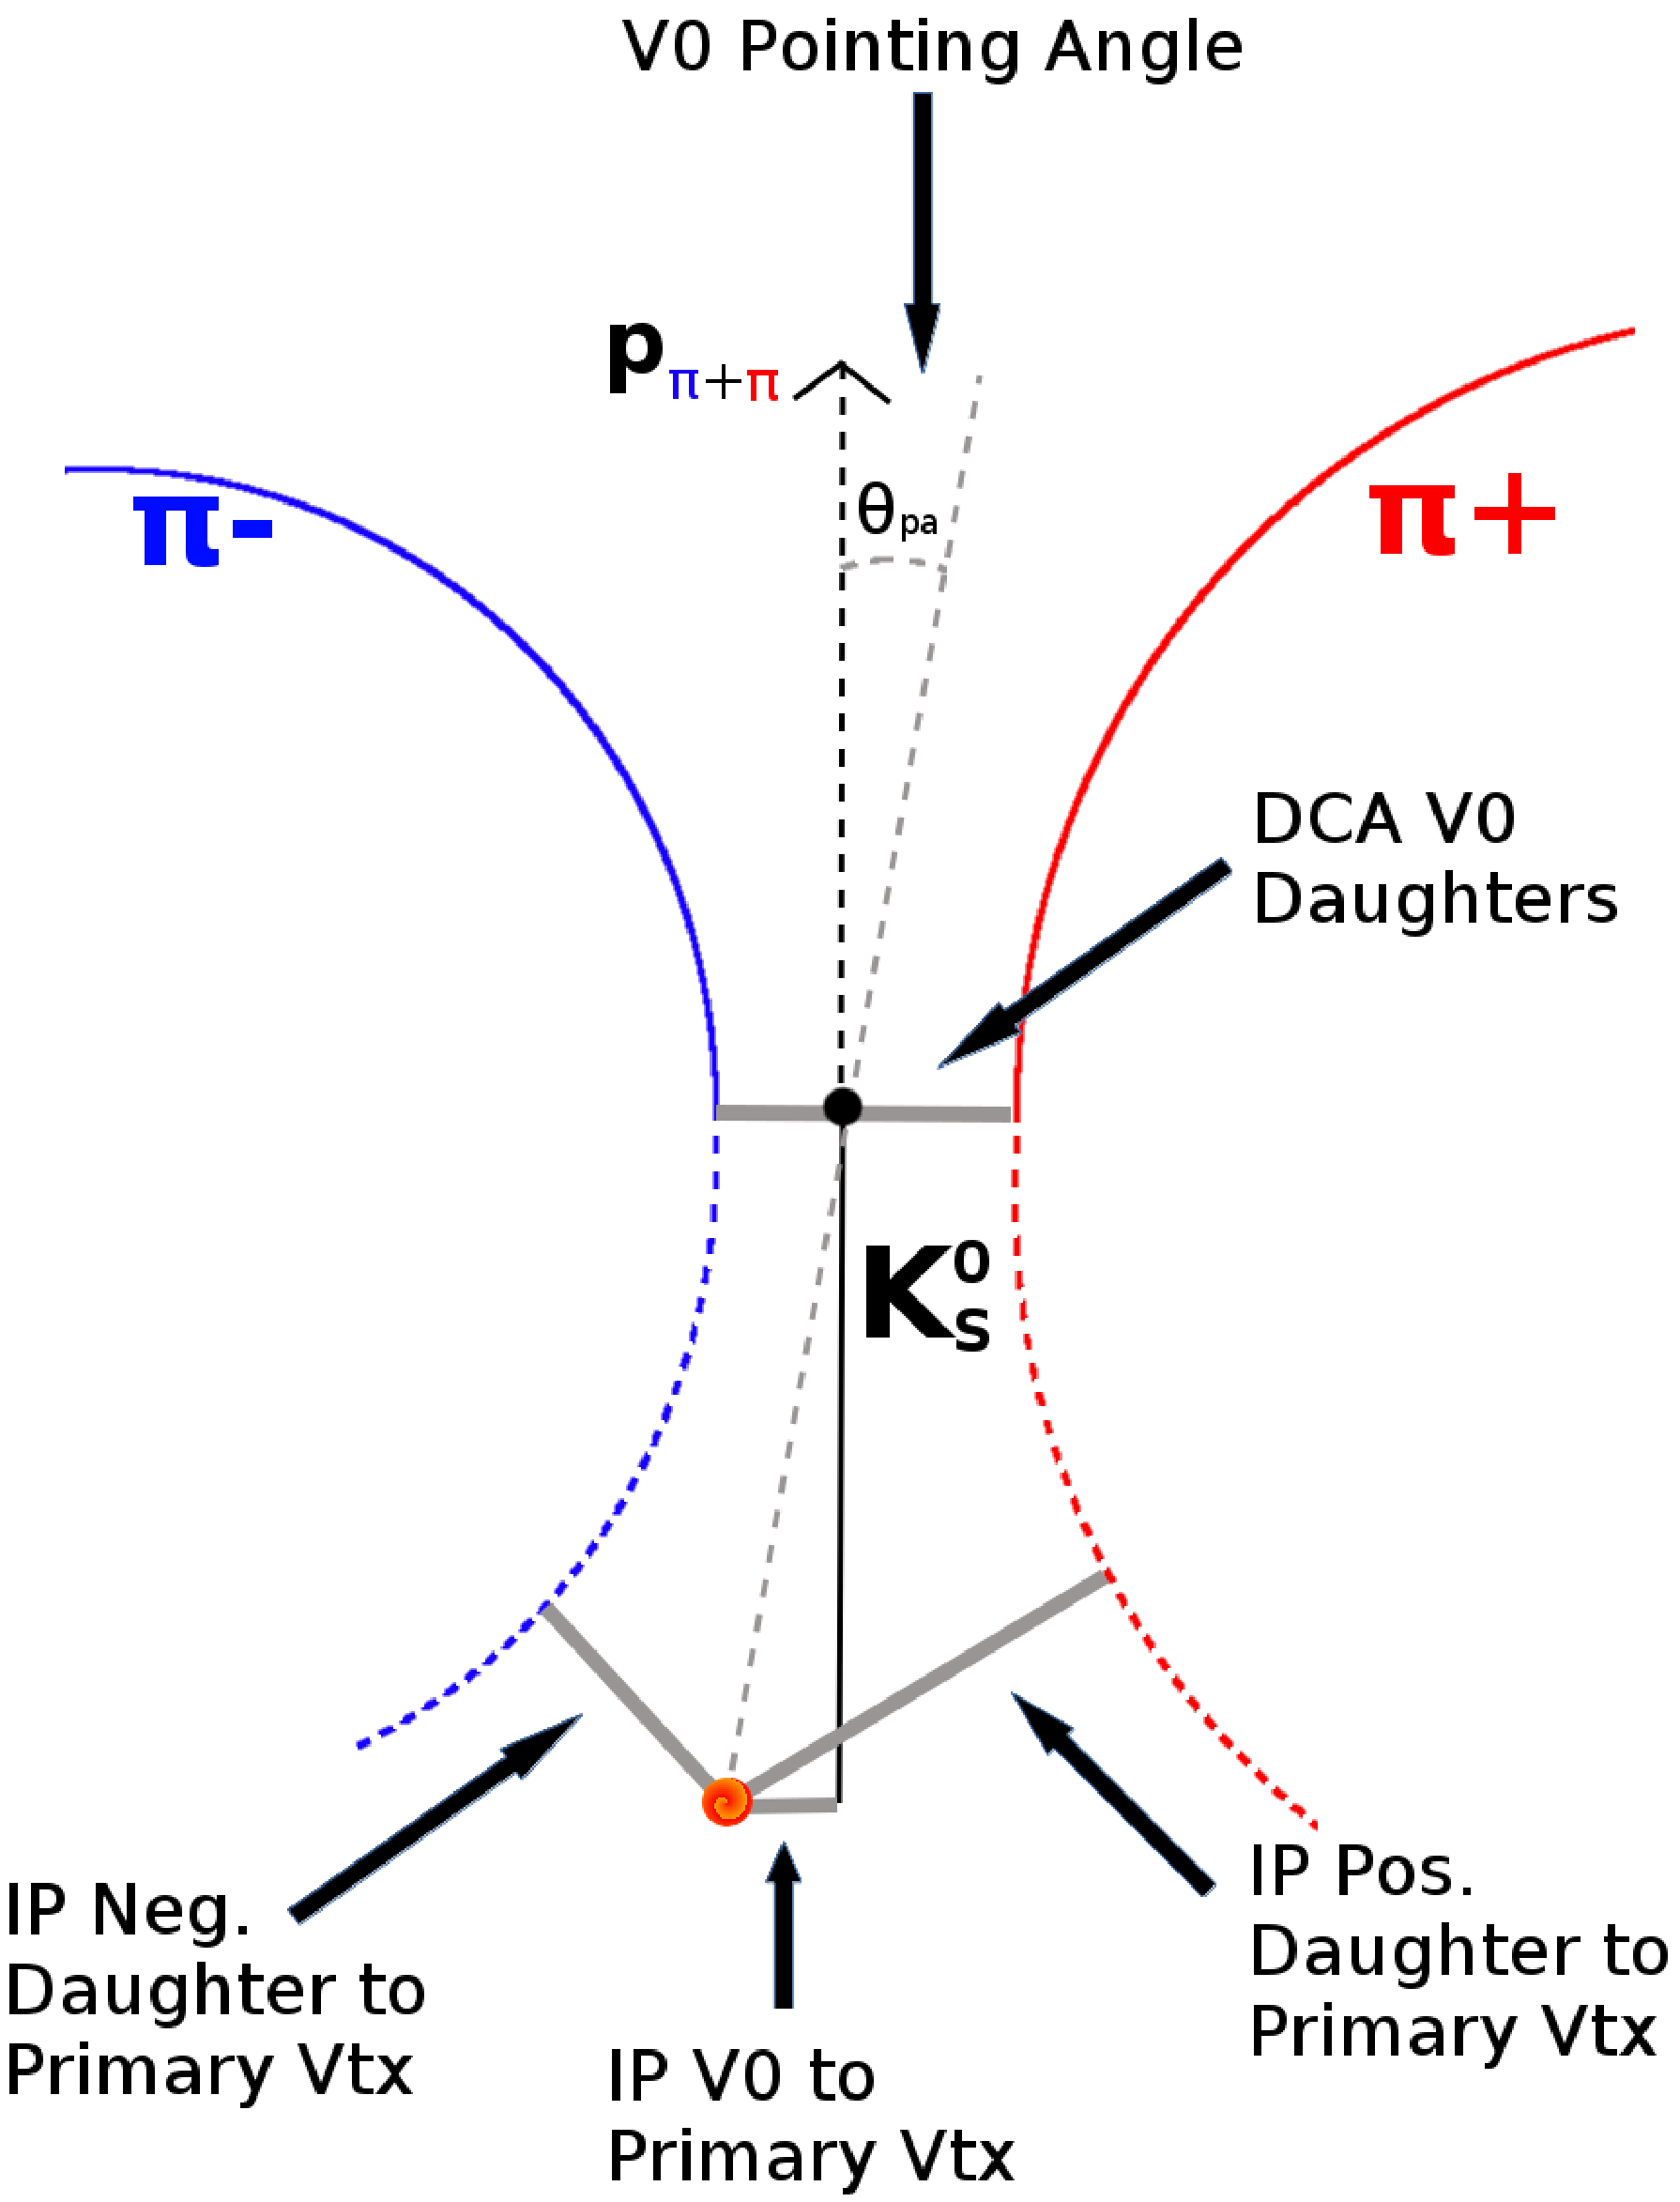
\includegraphics[width=18pc]{3_DataSelection/Figures/K0Cuts.pdf}
\end{minipage} 
\caption[Short Caption]{\label{fig:MomResLL} Long caption}
\end{figure}

\subfile{3_DataSelection/3.3.1_LambdaReconstruction.tex}
\subfile{3_DataSelection/3.3.2_K0sReconstruction.tex}

\end{document}
